\documentclass[10pt,a4paper]{article}
\usepackage[utf8]{inputenc}
\usepackage[T1]{fontenc}
\usepackage[spanish,es-noshorthands]{babel}
\usepackage[margin=3cm]{geometry}
\usepackage{amsmath,amssymb}
\usepackage{booktabs,tabularx,array}
\usepackage{enumitem}
\usepackage[most]{tcolorbox}
\usepackage{xcolor}
\usepackage{fancyhdr}
\usepackage{pdflscape}
\usepackage{graphicx}
\usepackage{caption}
\usepackage{subcaption}
\usepackage{float}
\usepackage{booktabs}
\usepackage{tabularx}
\usepackage{float}
\usepackage[colorlinks=true,linkcolor=blue!50!black,urlcolor=blue!50!black]{hyperref}

% Permite cortar las líneas después de los guiones bajos (nombres de funciones y ficheros largos)
\let\guionbajo\_
\renewcommand{\_}{\guionbajo\allowbreak}
\emergencystretch=2em

\begin{document}
\sloppy

\begin{titlepage}
    \centering
    \vfill
    {\huge \textbf{VISIÓN ARTIFICIAL POR APRENDIZAJE PROFUNDO} \par}
    \vspace{2cm}
    {\Large Proyecto: Clasificación de lesiones de piel. Del dermatoscopio a la foto de móvil. \par}
    \vspace{1cm}
    {\Large Universidad Autónoma de Madrid \par}
    \vspace{1cm}
    {\large Iván Domínguez Hernández |  ivan.dominguezh@estudiante.uam.es \par}
    \vspace{.5cm}
    {\large Lucas Miranda López | lucas.mirandal@estudiante.uam.es \par}
    \vspace{.5cm}
    {\large Niwei Chen | niwei.chen@estudiante.uam.es \par}
    \vspace{1cm}
\end{titlepage}

\tableofcontents

\newpage


\section{Introducción}

\noindent Este proyecto aborda la clasificación de lesiones de piel a partir de una imagen: dado un caso, el modelo debe decir
a qué diagnóstico corresponde (nevus, melanoma, carcinoma basocelular, queratosis, etc.). La motivación es un escenario
realista de cribado: los modelos suelen entrenarse con imágenes de dermatoscopio tomadas en hospitales, pero resultaría
útil poder usarlos con fotos hechas con un móvil, por ejemplo en atención primaria o en zonas sin especialista.

\medskip

\noindent Para reproducir ese escenario se usan dos conjuntos de datos públicos:

\begin{itemize}
    \item \textbf{Origen: HAM10000} (Tschandl et al., 2018). Reúne 10\,015 imágenes de dermatoscopio recogidas durante unos
    veinte años en la Universidad Médica de Viena (Austria) y en una consulta de Queensland (Australia). Cada imagen tiene uno
    de siete diagnósticos: queratosis actínica (\textit{akiec}), carcinoma basocelular (\textit{bcc}), queratosis benigna
    (\textit{bkl}), dermatofibroma (\textit{df}), melanoma (\textit{mel}), nevus (\textit{nv}) y lesión vascular
    (\textit{vasc}). Más de la mitad de los diagnósticos están confirmados por histopatología. Se usa la versión DermaMNIST
    de MedMNIST (Yang et al., 2023), que ofrece las imágenes reducidas a 128 píxeles y una partición oficial en
    entrenamiento, validación y test, pero no conserva ningún metadato del paciente ni de la lesión.
    \item \textbf{Destino: PAD-UFES-20} (Pacheco et al., 2020). Contiene 2\,298 fotos clínicas tomadas con distintos
    teléfonos móviles en el programa de dermatología de la Universidad Federal de Espírito Santo (Brasil), de 1\,373 pacientes
    y 1\,641 lesiones. Distingue seis diagnósticos: queratosis actínica (ACK), carcinoma basocelular (BCC), carcinoma
    escamoso (SCC), melanoma (MEL), nevus (NEV) y queratosis seborreica (SEK). Todos los cánceres de piel están confirmados
    por biopsia. Además de la imagen, cada caso incluye metadatos clínicos: edad, sexo, fototipo de Fitzpatrick, zona del
    cuerpo, tamaño de la lesión y síntomas como picor o sangrado. No trae particiones hechas.
\end{itemize}

\noindent Los dos conjuntos no usan exactamente las mismas clases ni registran la misma información, así que antes de
entrenar hay que emparejar sus diagnósticos y construir una tabla común con todas las imágenes (sección~\ref{sec:baseline}).

\medskip

\noindent Para resolver el problema planteado, se plantea una actuación en cuatro etapas:

\begin{enumerate}
    \item Construcción de un modelo de referencia (\textit{baseline}): un modelo
    preentrenado que no se modifica y, sobre sus características, un clasificador lineal.
    \item Aplicación de técnicas de aprendizaje con datos limitados. 
    \item Aplicación de técnicas de adaptación de dominio. 
    \item Análisis de comportamiento de los modelos.
\end{enumerate}

\noindent Todos los resultados se comparan con el modelo de referencia, por lo que la
preparación de los datos y la forma de medir se fijan en la primera etapa y no se cambian después.

\medskip

\noindent \textbf{Caso de uso:} parece lógico pensar que una app capaz de inferir un diagnóstico como apoyo a la decisión
con tan solo una imagen podría mejorar la vida de los profesionales en la atención primaria. Lógicamente 
no sería más que una ayuda, pues un sistema así sería de alto riesgo según la Ley de IA. Si bien esto no debería 
cambiar el foco del problema, que es el cambio de dominio de las imágenes, sería importante prestar atención al orden de 
magnitud, en inferencia, del tiempo que pueda tardar por imagen el modelo final. Quien sabe si en un futuro pudiera 
desarrollarse una tal aplicación, en colaboración con algún mecanismo de atención primaria o a nivel industrial. 

\newpage

\section{Baseline}
\label{sec:baseline}

\noindent En esta sección se encuentra todo aquello referente a la línea base.

\subsection{Adaptación de nuestros datos al baseline}

\noindent Lo más importante a comentar acerca de nuestro dataset:

\begin{enumerate}
    \item Separación de los datos en train, val, test: en test se deberían tener en cuenta solo datos nuevos. 
    La existencia de una fuga de datos, por tanto, supondría un problema: un mismo paciente no debería caer en 
    dos conjuntos distintos, pues de ser así no quedaría demostrado el hecho de que el modelo entrenado en train 
    generalice correctamente. 

    \begin{enumerate}
        \item Problema: HAM10000 (DermaMNIST) trae la partición hecha, y al descargar, guarda cada imagen en el directorio 
        correspondiente. DermaMNIST no guarda el identificador de lesión ni de paciente, así que no se puede comprobar si una 
        misma lesión ha caído en dos particiones. No lo podemos arreglar, solo documentarlo. Personalmente, daremos por hecho 
        que se está haciendo, pues es claro que es una buena práctica. 

        \item El dataset de destino, descargado de Hugging Face, PAD-UFES-20, no trae las particiones hechas, pero sí que trae el 
        id de cada paciente, por lo que si bien las particiones tendremos que hacerlas manualmente, evitar la fuga de datos está en 
        nuestra mano. 

        \item Aunque en la línea base no sea necesario, se han obtenido conjuntos de train, val y test tanto como para el dataset
        de origen como para el de destino, pues será necesario más adelante. En concreto: 

        \begin{center}
            \small
            \renewcommand{\arraystretch}{1.3}
            \begin{tabularx}{\linewidth}{@{}l>{\raggedright\arraybackslash}X>{\raggedright\arraybackslash}X@{}}
                \toprule
                & \textbf{Origen (dermatoscopio)} & \textbf{Destino (móvil)} \\
                \midrule
                \textbf{train} & Entrenar el \textit{linear probe} (baseline y U3)
                            & U4: adaptar el modelo con estas imágenes, sin etiquetas o con unas pocas. \\
                \textbf{val}   & Elegir modelo e hiperparámetros
                            & U4: elegir hiperparámetros de la adaptación \\
                \textbf{test}  & Medir cómo funciona en su propio dominio
                            & Medir cómo funciona en el dominio nuevo. \\
                \bottomrule
            \end{tabularx}
        \end{center}
    \end{enumerate} 

    \item Etiquetas: hay más etiquetas en el conjunto de origen (7) que en el de destino (6). Todas las etiquetas de destino están 
    correspondidas, con alguna etiqueta en origen. Para que las clases de destino ACK y SCC sean coherentes con alguna clase en origen,
    se han unificado en una única etiqueta, como se propone en el listado de temas para este conjunto de imágenes. De esta forma, técnicamente, 
    el destino tendría 5 clases, a corresponderse con 7 de origen. La intención del problema es clasificar las de destino, y de esta forma podemos 
    hacerlo. Sin embargo, los modelos serán entrenados con todas las clases en origen, pues el modelo tiene que estar entrenado de forma ciega con 
    respecto a su posterior uso. Dicho de otra forma, no deberíamos adaptar el conjunto en origen al de destino. Algunos comentarios acerca de las etiquetas:

    \begin{enumerate}

        \item Acerca del tratamiento de las etiquetas: no somos expertos en el dominio. Probablemente, lo mejor para tratarlas hubiera 
        sido consultar a un profesional y determinar si existe un estándar o si pudiera darnos consejo para hacerlo. Tal vez se podría 
        encapsular según qué etiquetas dentro de otras, al ser un tipo concreto de lesión cutánea un tipo particular de una más global. 
        No lo sabemos y queda pendiente en caso de ampliar el proyecto en un futuro. 

        \item La codificación de las etiquetas en origen se hace con números naturales: $\{c_i\}_{i=0}^6 = \{\}$. Y se hace que 
        correspondan, esas mismas etiquetas, en destino. Bajo estos índices, las etiquetas que se quedan sin representación son la 
        3 y la 6. Esta codificación es compatible con la funciones de pérdida que intuimos se usarán más adelante, como una cross-entropy, 
        que las tendrá en cuenta como índices.

    \end{enumerate} 
\end{enumerate}

\noindent Todo lo enumerado se recoge finalmente en la tabla común, como se ve a continuación:

\begin{center}
    \small
    \renewcommand{\arraystretch}{1.2}
    \begin{tabular}{@{}llrrrrrrrr@{}}
        \toprule
        \textbf{Dominio} & \textbf{Partición} & \textbf{akiec} & \textbf{bcc} & \textbf{bkl} & \textbf{df} & \textbf{mel} & \textbf{nv} & \textbf{vasc} & \textbf{Total} \\
        \midrule
        Dermatoscopio & train & 228 & 359 & 769 & 80 & 779 & 4693 & 99 & 7007 \\
                      & val   &  33 &  52 & 110 & 12 & 111 &  671 & 14 & 1003 \\
                      & test  &  66 & 103 & 220 & 23 & 223 & 1341 & 29 & 2005 \\
        \cmidrule(l){2-10}
                      & \textit{total} & 327 & 514 & 1099 & 115 & 1113 & 6705 & 142 & \textbf{10015} \\
        \midrule
        Móvil         & train & 554 & 507 & 141 & -- & 31 & 146 & -- & 1379 \\
                      & val   & 184 & 169 &  47 & -- & 11 &  49 & -- &  460 \\
                      & test  & 184 & 169 &  47 & -- & 10 &  49 & -- &  459 \\
        \cmidrule(l){2-10}
                      & \textit{total} & 922 & 845 & 235 & -- & 52 & 244 & -- & \textbf{2298} \\
        \midrule
        \multicolumn{2}{@{}l}{\textbf{Total}} & 1249 & 1359 & 1334 & 115 & 1165 & 6949 & 142 & \textbf{12313} \\
        \bottomrule
    \end{tabular}
\end{center}

\subsection{Exploración en los datos}

\noindent Una vez descargados, divididos en clases y conjuntos, en esta subsección se procederá con una exploración 
breve de los datos.

\medskip

\noindent \textbf{Desbalance de clase:}

\begin{center}
    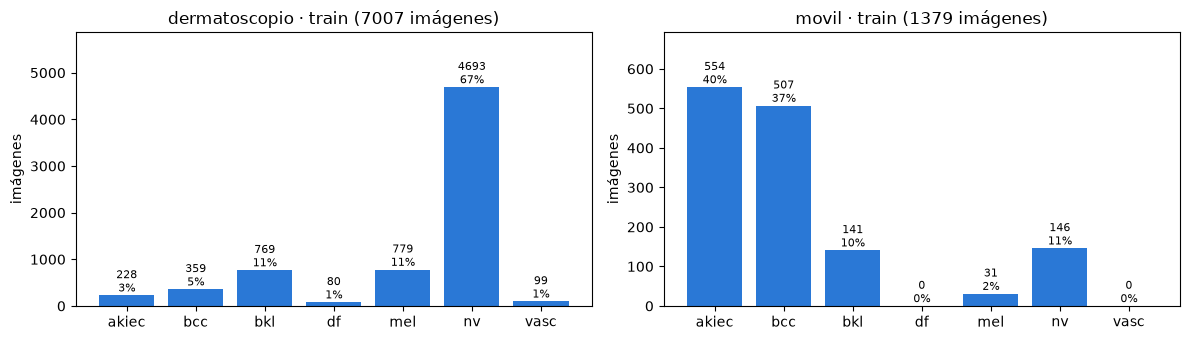
\includegraphics[width=\linewidth]{images/exploracion_1.png}
\end{center}

\noindent El desbalance de clases es más que evidente en train, tanto en el conjunto de origen como en el de destino. 
Esto, naturalmente, supondrá un problema a la hora de clasificar. Pero la idea es no tratarlo en el baseline, sino
en versiones más avanzadas del proyecto.

\medskip

\noindent \textbf{Sesgos en los datos:}

\medskip

\noindent En los metadatos del dataset de destino, se pueden asociar algunas 
imágenes con su valor en la escala de Fitzpatrick. Ésta recoge el tipo de piel
de cada paciente en función de como reacciona al sol. 
\begin{enumerate}
    \item Con fototipos I-II, la reacción es muy clara. Se quema siempre o casi siempre. 
    \item Con fototipos III-IV, encontramos pieles de intermedias a morenas claras.
    \item Con fototipos V-VI, pieles oscuras.
\end{enumerate}

\noindent Resumidamente, esto podría descubrir un posible sesgo de proporciones de nuestros datos, que en el peor de 
los casos podría implicar modelos que no funcionen correctamente en función del tipo de piel. Y esto tendría implicaciones 
raciales, por lo que necesariamente tendrá que ser una parte importante en secciones siguientes. El fototipo es desconocido
para el 35\% de las muestras. Además de la escala, también trae edad y sexo por paciente. Esto podrían también ser sesgos 
importantes a tener en cuenta. Una representación de los datos según estas categorías sería: 

\begin{center}
    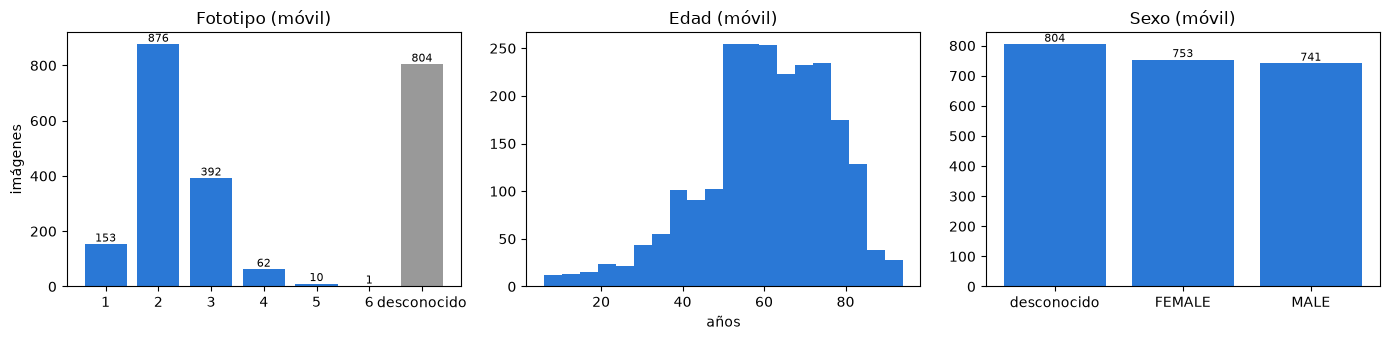
\includegraphics[width=\linewidth]{images/exploracion_2.png}
\end{center}

\noindent Algunas conclusiones:

\begin{enumerate}
    \item El 95\% están incluídas en los grupos I-III, lo que claramente implica un sesgo de representación en los datos, 
    como se comentaba antes. 
    \item Por suerte, esto no ocurre, en principio, para el sexo, como podemos observar. 
    \item En cuanto a la edad, parece seguir una distribución centrada entre los 50 y los 80 años, asimétrica hacia la izquierda. 
\end{enumerate}

\noindent Por tanto, es probable que más adelante haya que tratar tanto el sesgo de representación en los datos como
el referente a la edad. En nuestra opinión, sería un error eliminar fototipos poco  probables o desconocidos. 
Lo que proponemos es, en las conclusiones de equidad, solo tener en cuenta fototipos conocidos, mostrando 
especial atención en los minoritarios. 

\medskip

\noindent \textbf{Algunos ejemplos de cada clase en ambos dominios:}

\begin{center}
    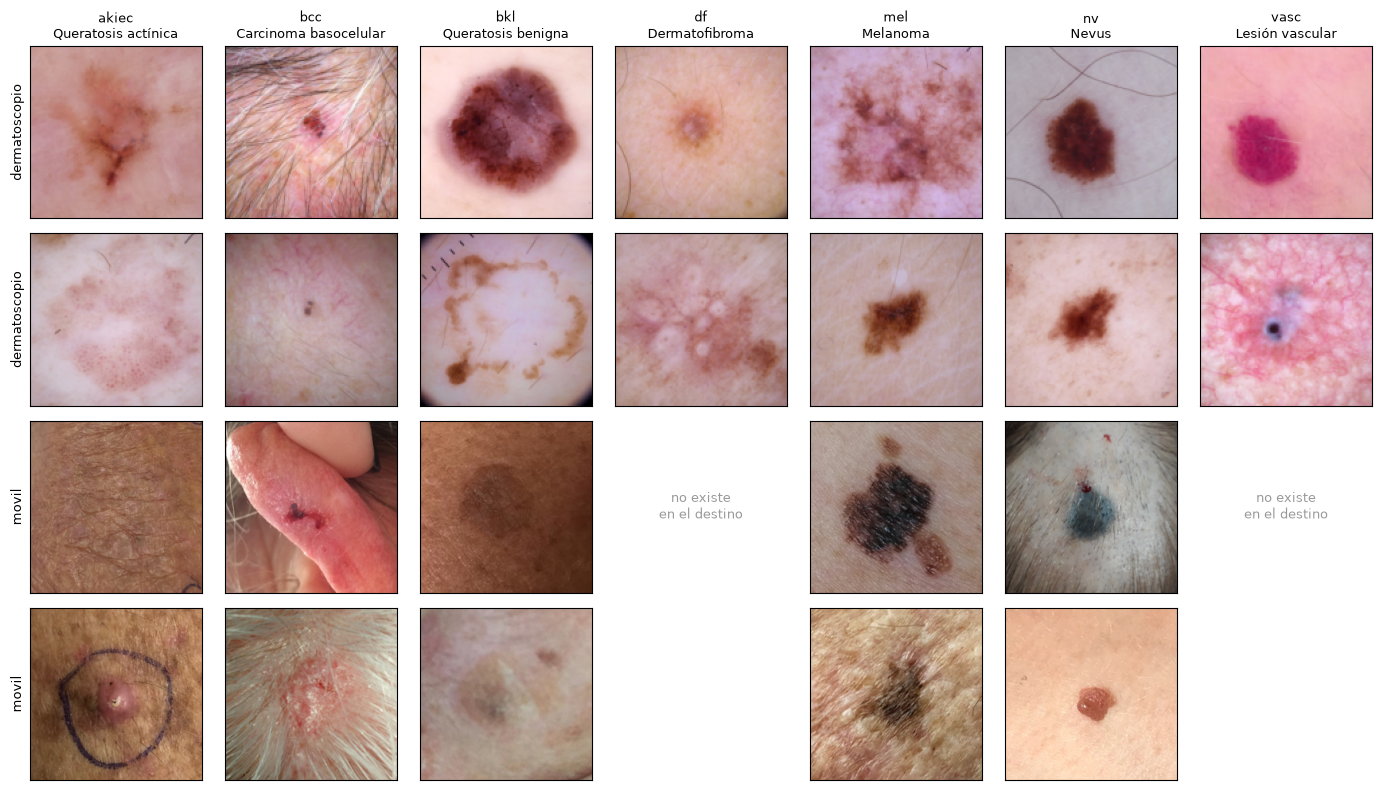
\includegraphics[width=\linewidth]{images/exploracion_3.png}
\end{center}

\subsection{Extracción de features}

\noindent La extracción de las features fue realizada de acuerdo con los
modelos propuestos en la plantilla de la línea base. En concreto, estos son ResNet50, 
DinoV2 (Meta - ViT) y CLIP (OpenAI - ViT). Queda pendiente, como se explica en la 
introducción, comprobar el orden de magnitud de tiempo en inferencia de estos modelos. 
Si fuera elevado, es probable que algún modelo ligero de la familia de MobileNet ofreciera
un balance adecuado entre precisión y velocidad en inferencia. Queda pendiente para el futuro. 

\subsection{Clasificador lineal}

\noindent Se entrena una capa lineal sobre cada una de las features obtenidas. Se obtienen,
para cada clasificador, en cada dominio y para cada partición (validación y test) el accuracy, el balanced 
accuracy y el Macro-F1. La tabla siguiente es orientativa de los resultados y es la referencia a batir
en U3 y U4:

\begin{center}
    \small
    \renewcommand{\arraystretch}{1.2}
    \begin{tabular}{@{}llrrrrrr@{}}
        \toprule
        & & \multicolumn{3}{c}{\textbf{Dermatoscopio}} & \multicolumn{3}{c}{\textbf{Móvil}} \\
        \cmidrule(lr){3-5} \cmidrule(l){6-8}
        \textbf{Modelo} & \textbf{Partición} & Acc. & Bal. acc. & Macro-F1 & Acc. & Bal. acc. & Macro-F1 \\
        \midrule
        ResNet-50     & val  & 0.722 & 0.577 & 0.519 & 0.222 & 0.315 & 0.219 \\
                      & test & 0.724 & 0.552 & 0.513 & 0.255 & 0.281 & 0.232 \\
        \midrule
        DINOv2 ViT-S/14 & val  & 0.765 & 0.578 & 0.551 & 0.333 & 0.306 & 0.242 \\
                        & test & 0.768 & \textbf{0.637} & \textbf{0.629} & \textbf{0.309} & \textbf{0.320} & \textbf{0.237} \\
        \midrule
        CLIP ViT-B/32 & val  & 0.795 & 0.650 & 0.632 & 0.198 & 0.292 & 0.200 \\
                      & test & \textbf{0.771} & 0.643 & 0.613 & 0.172 & 0.264 & 0.169 \\
        \bottomrule
    \end{tabular}
\end{center}

\noindent El Macro-F1 es la métrica que tiene en cuenta, no solo lo que el modelo
no es capaz de acertar (por ejemplo, la balanced accuracy tiene en cuenta $\frac{TP}{\text{\# objetos}}$), 
sino que también penaliza cuando falla, pues cuenta los falsos positivos. Por eso creemos que es la métrica que mejor 
puede tener en cuenta el hecho de que el modelo ataque al desbalance de clase, de ahí que sea nuestra métrica a tener en
cuenta a priori para comparar modelos y dominios. En concreto, obtenemos:

\begin{center}
    \small
    \renewcommand{\arraystretch}{1.2}
    \begin{tabular}{@{}lrrr@{}}
        \toprule
        \textbf{Modelo} & \textbf{Dermatoscopio} & \textbf{Móvil} & \textbf{Caída} \\
        \midrule
        ResNet-50       & 0.513 & 0.232 & 0.282 \\
        DINOv2 ViT-S/14 & 0.629 & 0.237 & 0.392 \\
        CLIP ViT-B/32   & 0.613 & 0.169 & 0.444 \\
        \bottomrule
    \end{tabular}
\end{center}

\noindent Podemos notar que el mejor modelo según esta métrica, es DINOv2. No es especialmente 
relevante, pues se está midiendo sobre train. Lo más relevante es que la caída de 
Macro-F1 al cambiar de dominio es bastante significativa. Por una parte, algo esperado, es el problema a tratar en siguientes
secciones. Por otra, bastante más alta de la que esperábamos, pensando en que realmente las lesiones son las mismas, o al
menos eso indican sus categorías. 

\subsection{Evaluación}

\noindent La selección del modelo se haría con el conjunto de validación en origen, pues la 
idea es seleccionar el mejor modelo, de nuevo, de forma ciega con respecto a su 
comportamiento en origen. Midiedo las métricas en validación, en el dominio del dermatoscopio, obtenemos
la siguiente tabla: 

\begin{center}
    \small
    \renewcommand{\arraystretch}{1.2}
    \begin{tabular}{@{}lrrr@{}}
        \toprule
        \textbf{Modelo} & \textbf{Accuracy} & \textbf{Bal. acc.} & \textbf{Macro-F1} \\
        \midrule
        \textbf{CLIP ViT-B/32} & \textbf{0.795} & \textbf{0.650} & \textbf{0.632} \\
        DINOv2 ViT-S/14        & 0.765 & 0.578 & 0.551 \\
        ResNet-50              & 0.722 & 0.577 & 0.519 \\
        \bottomrule
    \end{tabular}
\end{center}

\noindent En concreto, en nuestro caso, la selección del mejor modelo en validación es sencilla, pues el que parte de CLIP
parece ser bastante superior en todas las métricas que hemos medido. Concretamente, para este modelo, las métricas más 
relevantes acerca de su rendimiento de test, en ambos dominios, son las que siguen:

\begin{center}
    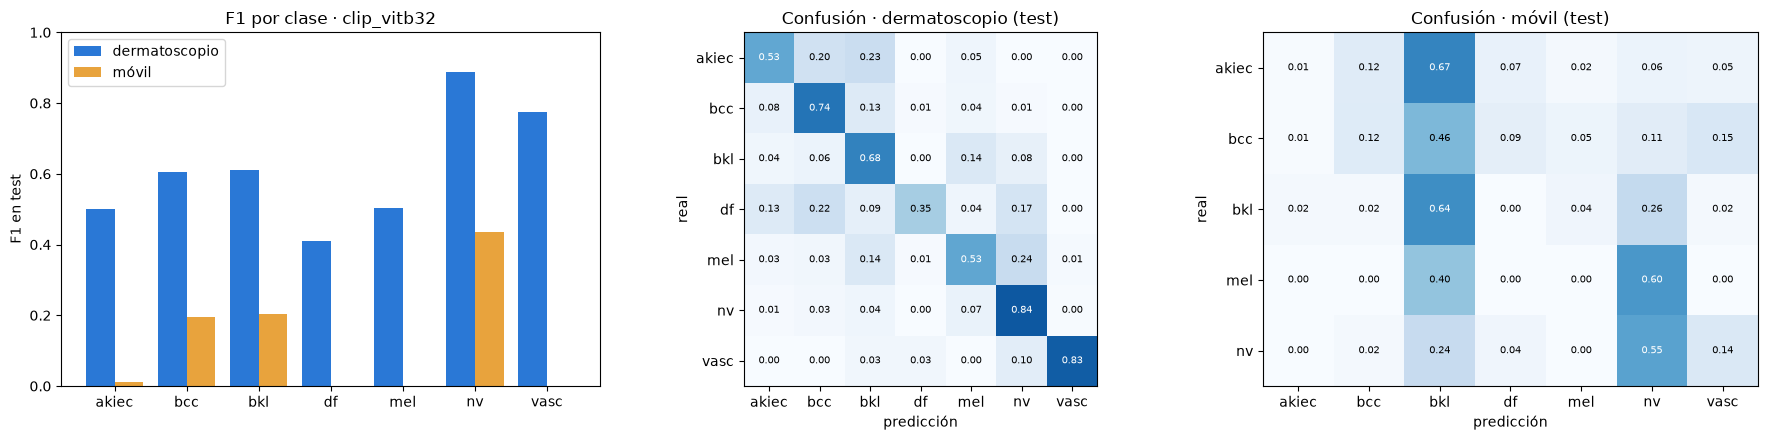
\includegraphics[width=\linewidth]{images/evaluacion_1.png}
\end{center}

\begin{enumerate}
    \item Su F1 en el dermatoscopio es alto incluso en algunas clases infrarepresentadas, como vasc, que representa menos 
    de un 1\% de los datos de train en el dermatoscopio. 
    \item Su F1 en el móvil es un auténtico desastre. Lo achacamos al cambio de dominio, aunque descubriremos otras causas 
    más adelante. 
    \item La matriz de confusión en el dermatoscopio es un ejemplo de cómo debería lucir, a simple vista, una matriz de confusión: una diagonal
    de color azul. Esto es una buena señal. Si bien algunas clases tienen accuracys bajos, sigue siendo un buen resultado para un baseline. 
    \item No podemos decir lo mismo para la matriz de confusión al cambiar de dominio, donde la diagonal no está ni marcada. Está lejos 
    de lo que debería. 
\end{enumerate}

\noindent Podemos añadir un análisis de equidad con respecto a los resultados de test en el dominio del móvil. Para ello, 
tendremos en cuenta (en azul), tan solo el accuracy que tengan aquellos grupos con más de 30 imágenes:

\begin{center}
    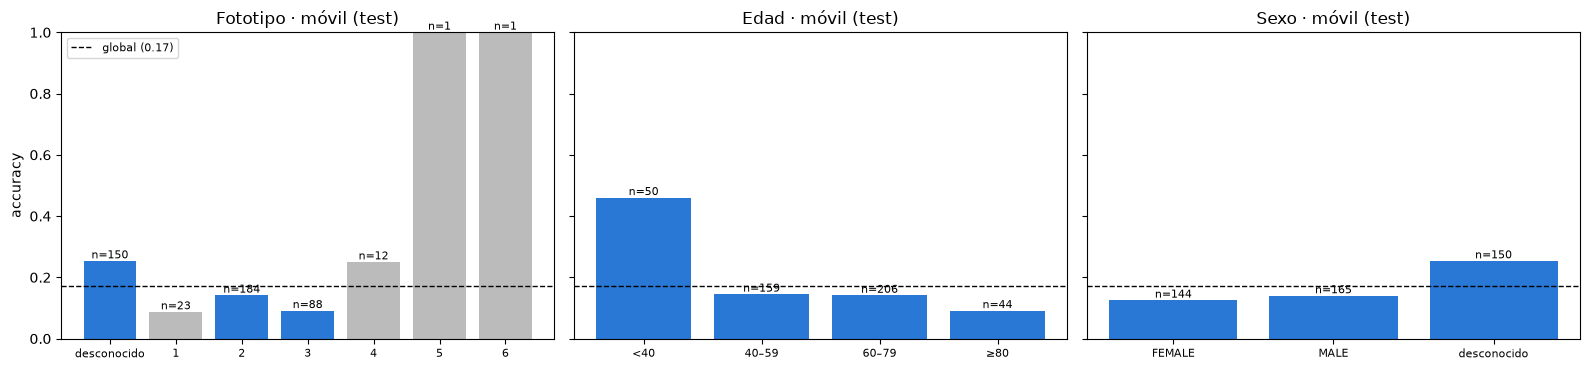
\includegraphics[width=\linewidth]{images/evaluacion_2.png}
\end{center}

\noindent Algunos comentarios acerca de estos resultados:

\begin{enumerate}
    \item El accuracy relativo a los fototipos conocidos y con representación razonable no está demasiado desbalanceado. 
    El hecho de que acierte siempre las lesiones de personas de fototipos V-VI se comentará más abajo. 

    \item Sí que parece que el modelo tiene mayor facilidad de acertar las lesiones de piel de personas jóvenes ($\leq 40$) que las 
    de mayor edad. Esto se puede justificar argumentando que las arrugas dificultan el hecho de predecir lesiones de piel, pues podemos 
    entender las arrugas como ruido como tal. Sin embargo, visto desde otra óptica, puede ser que las clases de lesiones de piel sean más
    fáciles de predecir para rangos de edad más jóvenes. El hecho de que el tipo de lesión sea distinto según el grupo de la edad es una 
    explicación sencilla, bajo el supuesto de que el rango de edad puede determinar el tipo de lesión de piel que se tenga, especialmente 
    con lesiones como el melanoma. Se comprueba un poco más abajo. 

    \item El modelo predice también igual de bien independientemente del sexo. 
\end{enumerate}

\noindent \textbf{Acerca de los tipos de lesión según el fenotipo de piel:}

\medskip

\noindent El hecho de que que predigan tan bien las muestras de los fotitipos V y VI podría no parecer relevante dado que hay tan pocas muestras. 
Aún así, se propone investigar cuales son las clases en train de esos fototipos para averiguar si las predicciones son invariantes al fototipo. 
Encontramos lo siguiente:

\begin{center}
    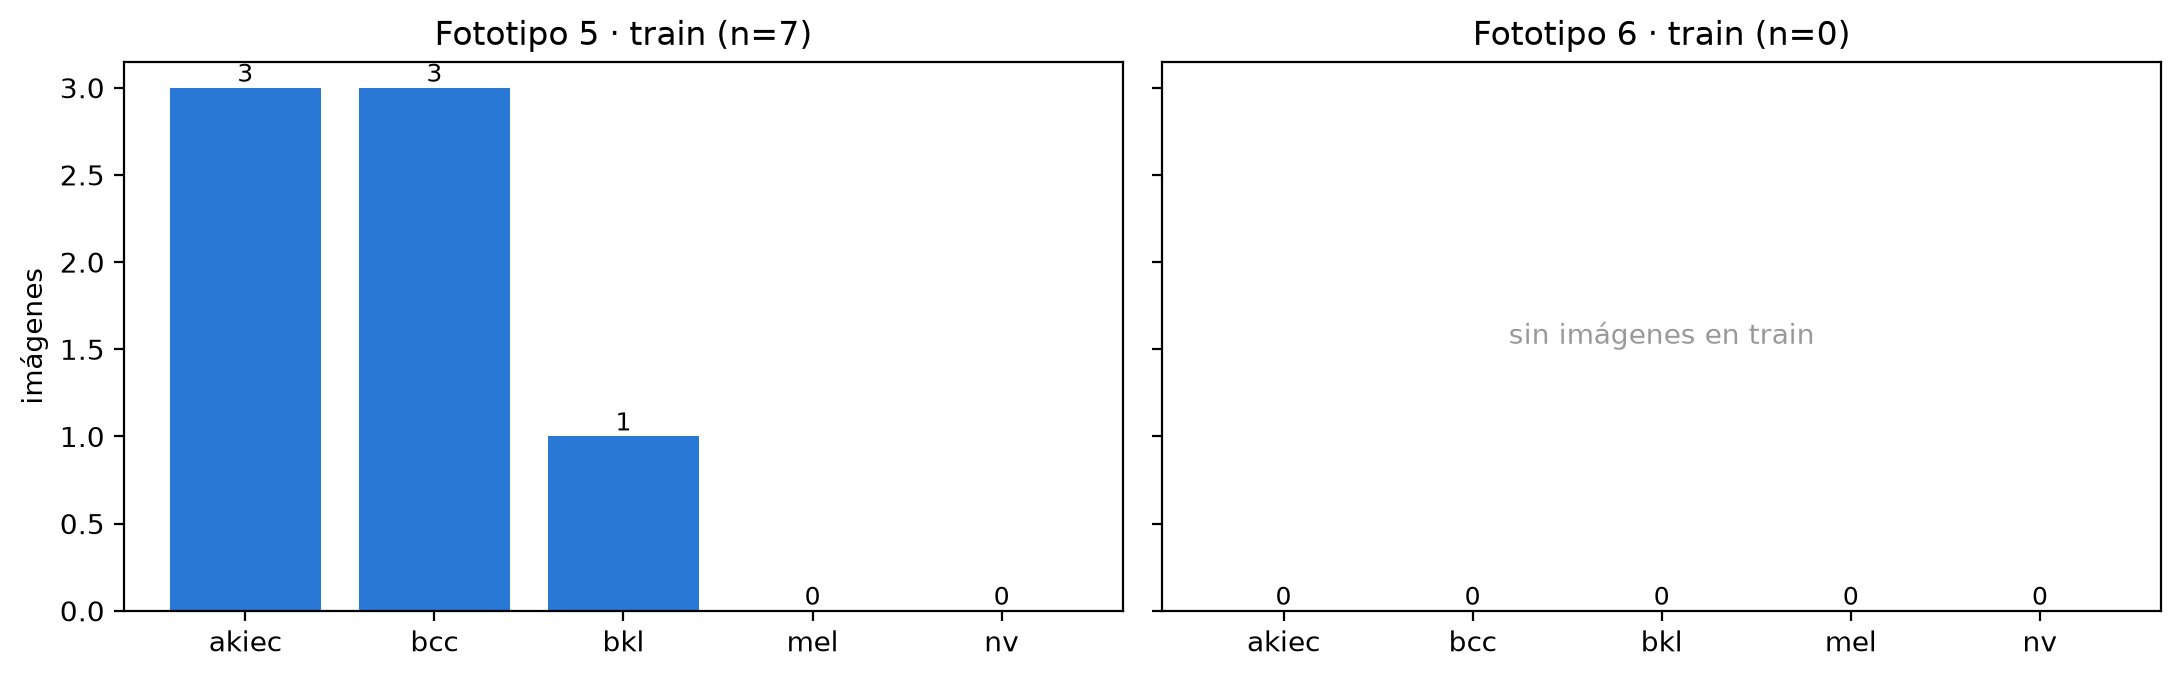
\includegraphics[width=\linewidth]{images/revision_fototipos56_train.png}
\end{center}

\noindent En validación y test, son:

\begin{center}
    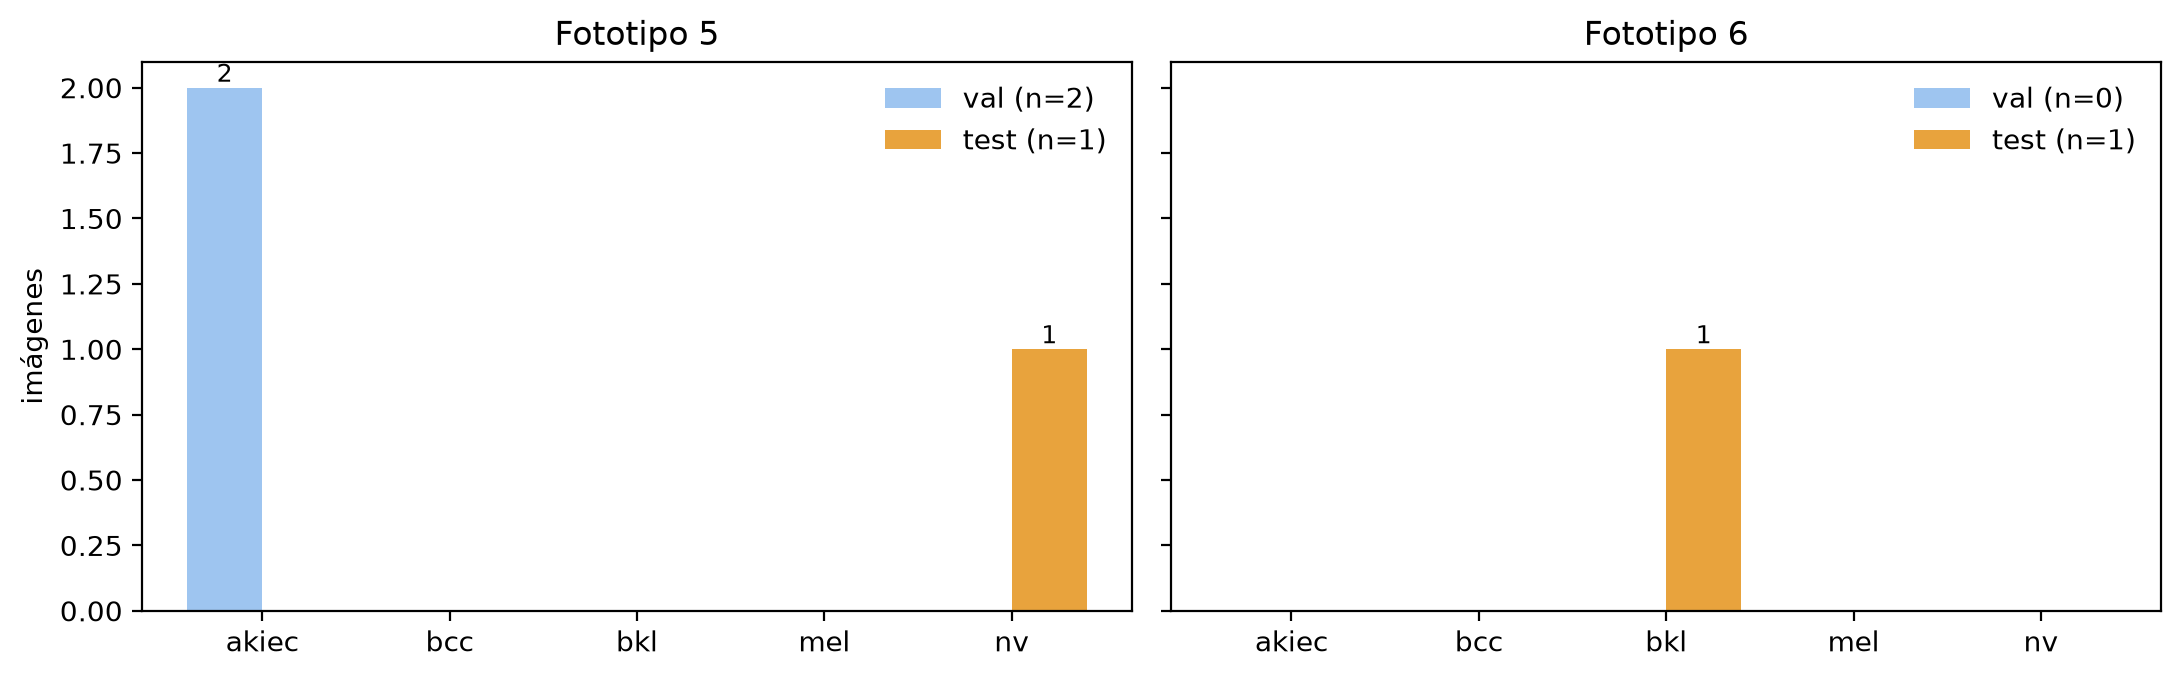
\includegraphics[width=\linewidth]{images/revision_fototipos56_val_test.png}
\end{center}

\noindent Si bien esto es difícil de interpretar, lo que sí que sabemos es que el modelo, sin ver nunca en train una imagen de un 
fototipo VI, es capaz de acertarlo en test. Algo parecido pasa cpn el fototipo V, que si bien sí que ve en el conjunto de train, 
creemos que no lo suficiente como para aprender a distinguirlo. No hay evidencia suficiente como para afirmar que el modelo generalice
bien sin importar el fototipo, pero con los datos que tenemos, desde luego, es todo lo que podemos decir. 

\medskip

\noindent No estaría de más, más adelante, tener cuidado con las partes de la imagen en las que se fija el modelo cuando se trata de 
estos fenotipos via algoritmos como Grad-CAM. Es posible que, de cara a hacer las predicciones, se base antes en el tipo de piel que 
en la lesión en sí, lo que querría decir que el modelo no aprende lo que se pretente. Aunque esto no cuadra demasiado con los resultados, 
puesto que en train ve más de una sola lesión para el fenotipo V (y las clases predichas ni si quiera cuadran con las clases que ve en train) 
y ninguna para el VI, lo revisaremos más adelante. 

\medskip

\noindent \textbf{Acerca de las lesiones según los rangos de edad:}

\medskip

\noindent Parece evidente el hecho de que habrá según qué rangos de edad predispuestos a según qué lesiones algo que puede
explicar que el modelo prediga mejor las lesiones para grupos de edad más jóvenes. Podemos comprobarlo:

\begin{center}
    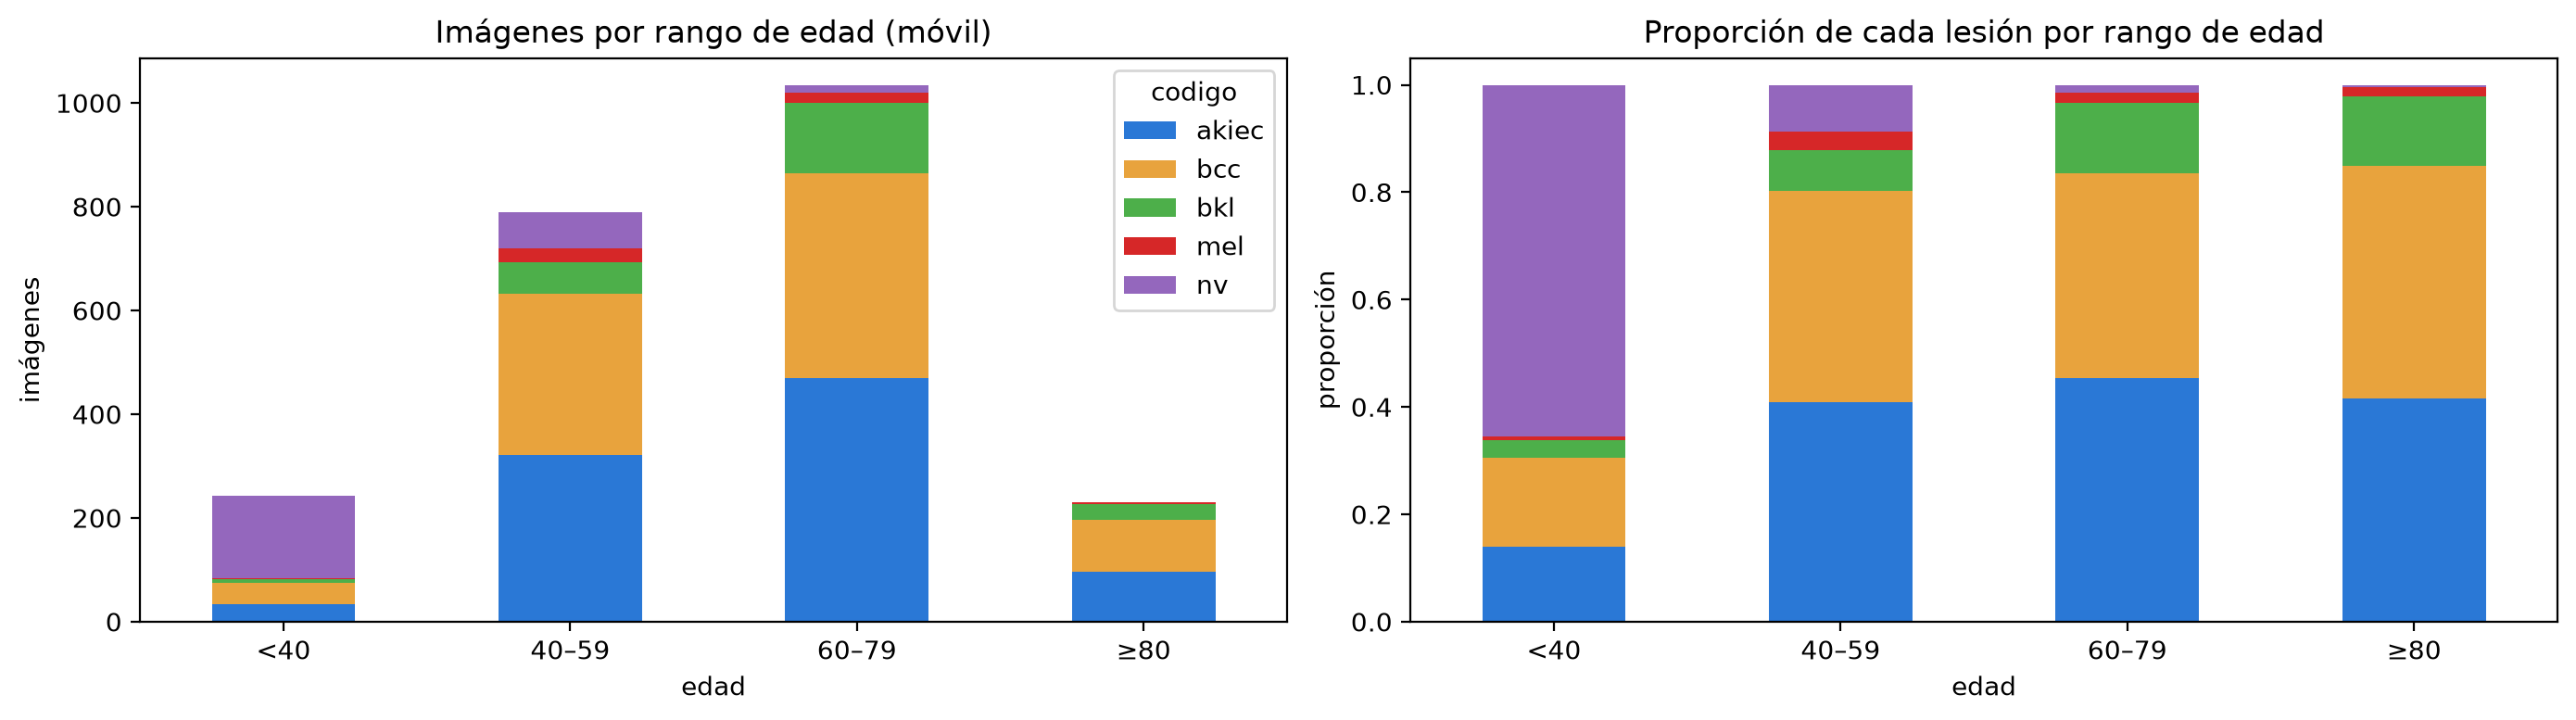
\includegraphics[width=\linewidth]{images/revision_lesiones_por_edad.png}
\end{center}

\noindent Como era de esperar, la distribución de lesiones según el rango de edad varía bastante. No hay mucho que hacer en esta sección, 
más que constatarlo para tenerlo en cuenta más adelante. Sin embargo, el hecho de que cambie la distribución no tiene por qué significar 
que el modelo las aprenda peor. En concreto, los accuracy por clase y rango de edad son los siguientes:

\begin{center}
    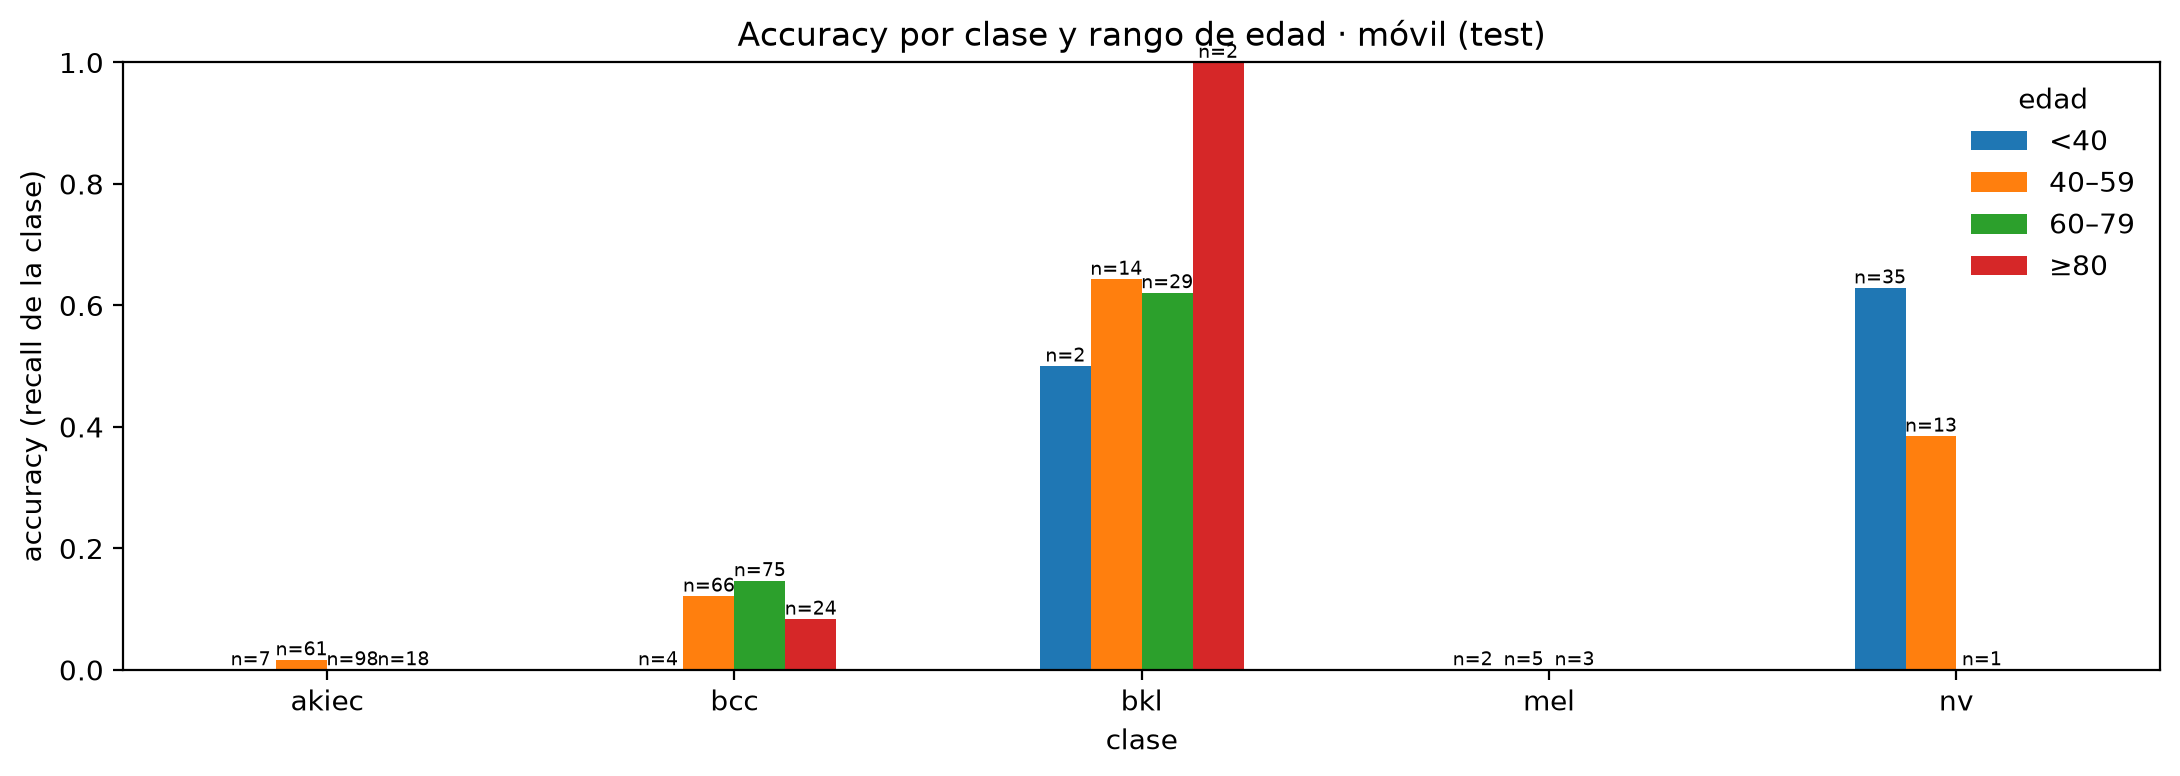
\includegraphics[width=\linewidth]{images/revision_accuracy_clase_edad.png}
\end{center}

\noindent En conclusión: a vista de estos resultados podemos, si bien no constatarlas, sí obtener algunas conclusiones que 
pudieran ser intuitivas. No hay datos suficientes para afirmar que los modelos predicen mejor para según que fototipos de 
piel. La evidencia que tenemos es que, sin embargo, sí que parecen predecir mejor en función del rango de edad, pero esto
no se debe, o al menos no hay evidencia para creerlo, a que las imágenes sean más o menos sencillas, sino a que la distribución de 
lesiones por rango de edad varía. Y por último, también parece que las predicciones no mejoran ni empeoran en función del sexo, pues 
el dataset no presenta sesgo en este sentido. 

\medskip

\noindent Es probable que, una de las formas de tratar estos problemas más adelante, sea construir batches balanceados que permitan 
al modelo ver, en cada época, lotes de imágenes coherentemente distribuidas. Queda pendiente para secciones siguientes.

\subsection{Otras cuestiones relevantes}

\begin{enumerate}
    \item \textbf{Cantidad de datos:} existen datos suficientes. A pesar del desbalance de clases, podemos afirmar esto, especialmente
    teniendo en cuenta que la idea del proyecto es tratar el desbalance, entrenar los modelos con pocos
    datos. Algunos ejemplos de clases, dentro de dominios, infrarrepresentadas, a continuación:
    \begin{center}
    \small
    \renewcommand{\arraystretch}{1.2}
    \begin{tabular}{@{}llrrrr@{}}
        \toprule
        \textbf{Dominio} & \textbf{Clase} & \textbf{train} & \textbf{val} & \textbf{test} & \textbf{\% del train} \\
        \midrule
        Dermatoscopio & df (dermatofibroma)      &  80 & 12 & 23 & 1.1\,\% \\
                      & vasc (lesión vascular)   &  99 & 14 & 29 & 1.4\,\% \\
                      & akiec (queratosis act.)  & 228 & 33 & 66 & 3.3\,\% \\
        \midrule
        Móvil         & mel (melanoma)           &  31 & 11 & 10 & 2.2\,\% \\
                      & bkl (queratosis benigna) & 141 & 47 & 47 & 10.2\,\% \\
        \bottomrule
    \end{tabular}
\end{center}

    \item \textbf{Modelo de mejor rendimiento}
    \begin{enumerate}
        \item CLIP es el mejor en validación.
        \item DINOv2 es el mejor en test.
        \item ResNet es el peor en el origen.
        \item CLIP es el peor en el móvil.
    \end{enumerate}
    Nos hemos quedado con CLIP, pues siguiendo buenas prácticas, es el que mejor rendimiento aporta en el
    conjunto de validación en el dermatoscopio. 
    \item \textbf{Las clases de peor rendimiento:} no necesariamente son las de menor representación. Como vimos antes, vasc tiene un F1 alto en el dermatoscopio. 
    Un análisis breve acerca de las clases de peor rendimiento: 
    \begin{center}
    \small
    \renewcommand{\arraystretch}{1.2}
    \begin{tabular}{@{}lrrrl@{}}
        \toprule
        \textbf{Clase} & \textbf{Imág. train} & \textbf{F1} & \textbf{Recall} & \textbf{Se confunde sobre todo con} \\
        \midrule
        df (dermatofibroma)     &  80 & 0.41 & 0.35 & bcc (0.22), nv (0.17), akiec (0.13) \\
        akiec (queratosis act.) & 228 & 0.50 & 0.53 & bkl (0.23), bcc (0.20) \\
        mel (melanoma)          & 779 & 0.50 & 0.53 & nv (0.24), bkl (0.14) \\
        \bottomrule
    \end{tabular}
    \end{center}
    \item \textbf{Diferentes dominios:} hay diferentes dominios, claramente, y se diferencian en dos cosas a la vez. 
    \begin{enumerate}
        \item  La \textbf{imagen}: el dermatoscopio da imágenes ampliadas,
        centradas y con luz uniforme, mientras que las fotos de móvil tienen más piel alrededor, luz variable y otro encuadre
        (ver los ejemplos de la exploración). 
        \item  Las \textbf{proporciones de clases}: \textit{nv} pasa de ser el
    67\,\% del origen al 11\,\% del móvil, y \textit{akiec} y \textit{bcc} pasan de un 3--5\,\% a casi el 80\,\% entre las dos.
    \end{enumerate}

    \begin{center}
        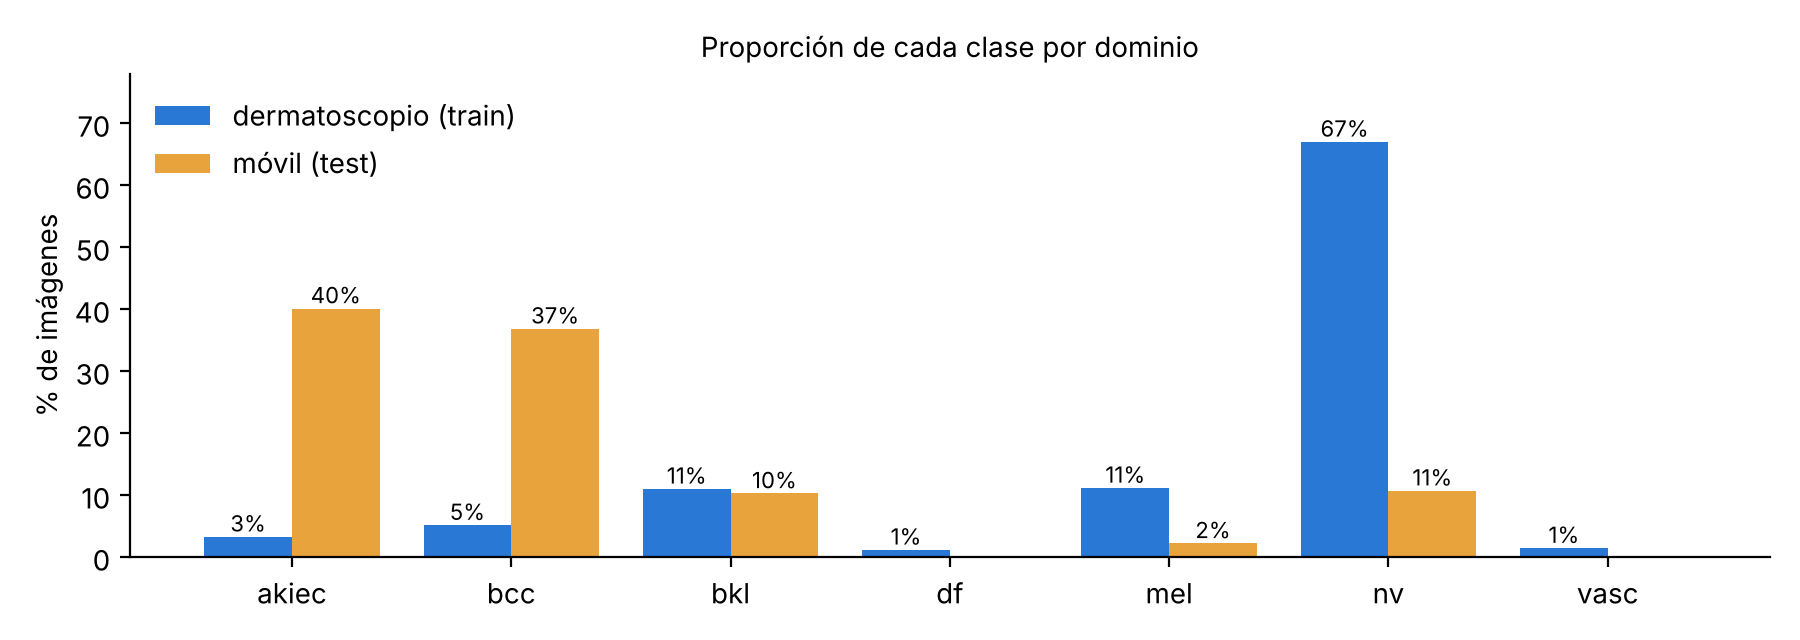
\includegraphics[width=\linewidth]{images/dominios_proporciones.png}
    \end{center}

    \item \textbf{Sensibilidad:} se trata de un tema sensible, por varios motivos:
    \begin{enumerate}
        \item \textbf{Son datos de salud}, una categoría especialmente protegida. Ejecutar el modelo en el propio teléfono,
        como se plantea en la introducción, evita que las fotos de los pacientes salgan del dispositivo.
        \item \textbf{Los errores tienen consecuencias graves.} Un melanoma clasificado como nevus retrasa el diagnóstico de
        un cáncer, y un falso positivo provoca pruebas innecesarias. Por eso el sistema solo debería plantearse como
        \textbf{apoyo a la decisión} (sugerir qué lesiones derivar al dermatólogo), nunca como diagnóstico, y la decisión
        final debe tomarla un profesional.
        \item \textbf{Según la Ley de IA europea sería un sistema de alto riesgo}, al tratarse de software con fines
        médicos. Eso exige, entre otras cosas, documentar los datos y sus limitaciones, supervisión humana y evaluar su
        rendimiento antes de usarlo.
        \item \textbf{Equidad.} Casi no hay imágenes de pieles oscuras (fototipos IV--VI), así que no se puede saber si el
        modelo funciona igual para ellas. Usarlo en una población más diversa sin validarlo antes sería un riesgo.
    \end{enumerate}
\end{enumerate}
\end{document}